\subsection{Optimizing the Blended-Wing-Body Aircraft}
\label{ch5:sec:cs3}

We now demonstrate DeepGeo's capability to handle complex 3D geometries without tuning. To this end, we focus on optimizing the first-generation Boeing Blended-Wing-Body (BWB) design as shown in Fig.~\ref{ch5:fig:cs3_template_mesh}. The BWB aircraft configuration integrates the wing and fuselage into a single, seamless structure to enhance aerodynamic efficiency, reduce drag, and lower fuel consumption. The BWB used in this case study has a span of 280 feet, a total length of 144 feet and is designed to carry 800 passengers~\cite{aa.Liebeck2004}.
A notable challenge in this design is that the supersonic airflow creates significant shock waves, introducing strong drag forces. The key to optimization is refining the BWB shape to mitigate these drag-inducing effects.

\begin{table}[!b]
  \centering
  \caption{\small Aerodynamic shape optimization task specifications for the Case Study III.}
  \resizebox{1\columnwidth}{!} {
        \begin{tabular}{lllrr}
        \hline
        \multicolumn{1}{l}{\textbf{Objectives}} & \textbf{Functions/Variables} & \textbf{Description} & \multicolumn{1}{l}{\textbf{DeepGeo Quantity}} & \multicolumn{1}{l}{\textbf{FFD Quantity}} \\
        \hline
        \multicolumn{1}{l}{\textbf{Minimize}} & $C_D$  & Drag coefficient &        &  \\
        \hline
        \multicolumn{1}{l}{\multirow{3}[2]{*}{\textbf{With respect to}}} & $\Theta$ & Weights of DeepGeo & \num{151585} &         \\
        \multicolumn{1}{l}{} & $P_z$  & Control points' $z$ coordinates &        & 240 \\
        \multicolumn{1}{l}{} & $\alpha$ & Angle of attack & 1      & 1 \\
        \hline
        \multicolumn{3}{l}{\textbf{Total design variables}} & \num{151586} & 241 \\
        \hline
        \multicolumn{1}{l}{\multirow{5}[2]{*}{\textbf{Subject to}}} & $C_L=0.20056$ & Lift coefficient constraint & 1      & 1 \\
        \multicolumn{1}{r}{} & $C_M=0$ & Moment coefficient constraint & 1      & 1 \\
        \multicolumn{1}{r}{} & $t \ge 0.01 \; t_\text{original}$ & Minimum thickness constraints &        & 750 \\
        \multicolumn{1}{r}{} & $Vol \ge {Vol}_\text{original}$ & Minimum volume constraint & 1      &  1 \\
        \multicolumn{1}{r}{} & $0 \leq \alpha \leq 2.5$ & Angle of attack constraint & 1      &  1 \\
        \hline
        \multicolumn{3}{l}{\textbf{Total constraints}} & 7      & 754 \\
        \hline
        \multicolumn{3}{l}{\textbf{Need value range limits for each DV?}} & NO     & YES \\
        \hline
        \end{tabular}%
    }
  \label{ch5:tab:bwb_DV_cons}%
\end{table}%

\subsubsection{Problem Formulation}

The optimization objective is to minimize the drag coefficient $C_D$ while constraining the lift coefficient $C_L$ to $0.20056$ and ensuring a pitching moment coefficient $C_M$ of 0. This single-point optimization problem is performed under fully turbulent flow conditions at a Mach number of $0.85$, Reynolds number of $5\times10^6$ and an initial angle of attack of $0.58^{\circ}$. The optimization is performed on both the mesh that has $1,070,080$ cells, corresponding to the same setting as the L2 grid configuration in~\citet{aa.Lyu2014}. Shape modifications are allowed only along the $z$ axis to maintain a constant projected area, and the aircraft volume is constrained to remain above its initial value, preventing shrinkage that could reduce drag but compromise capacity. Compared to the optimization task of the CRM wing, the task for BWB aircraft is less constrained. Tab.~\ref{ch5:tab:bwb_DV_cons} summarizes the experimental setup. 

\begin{figure}[ht]
    \begin{center}
        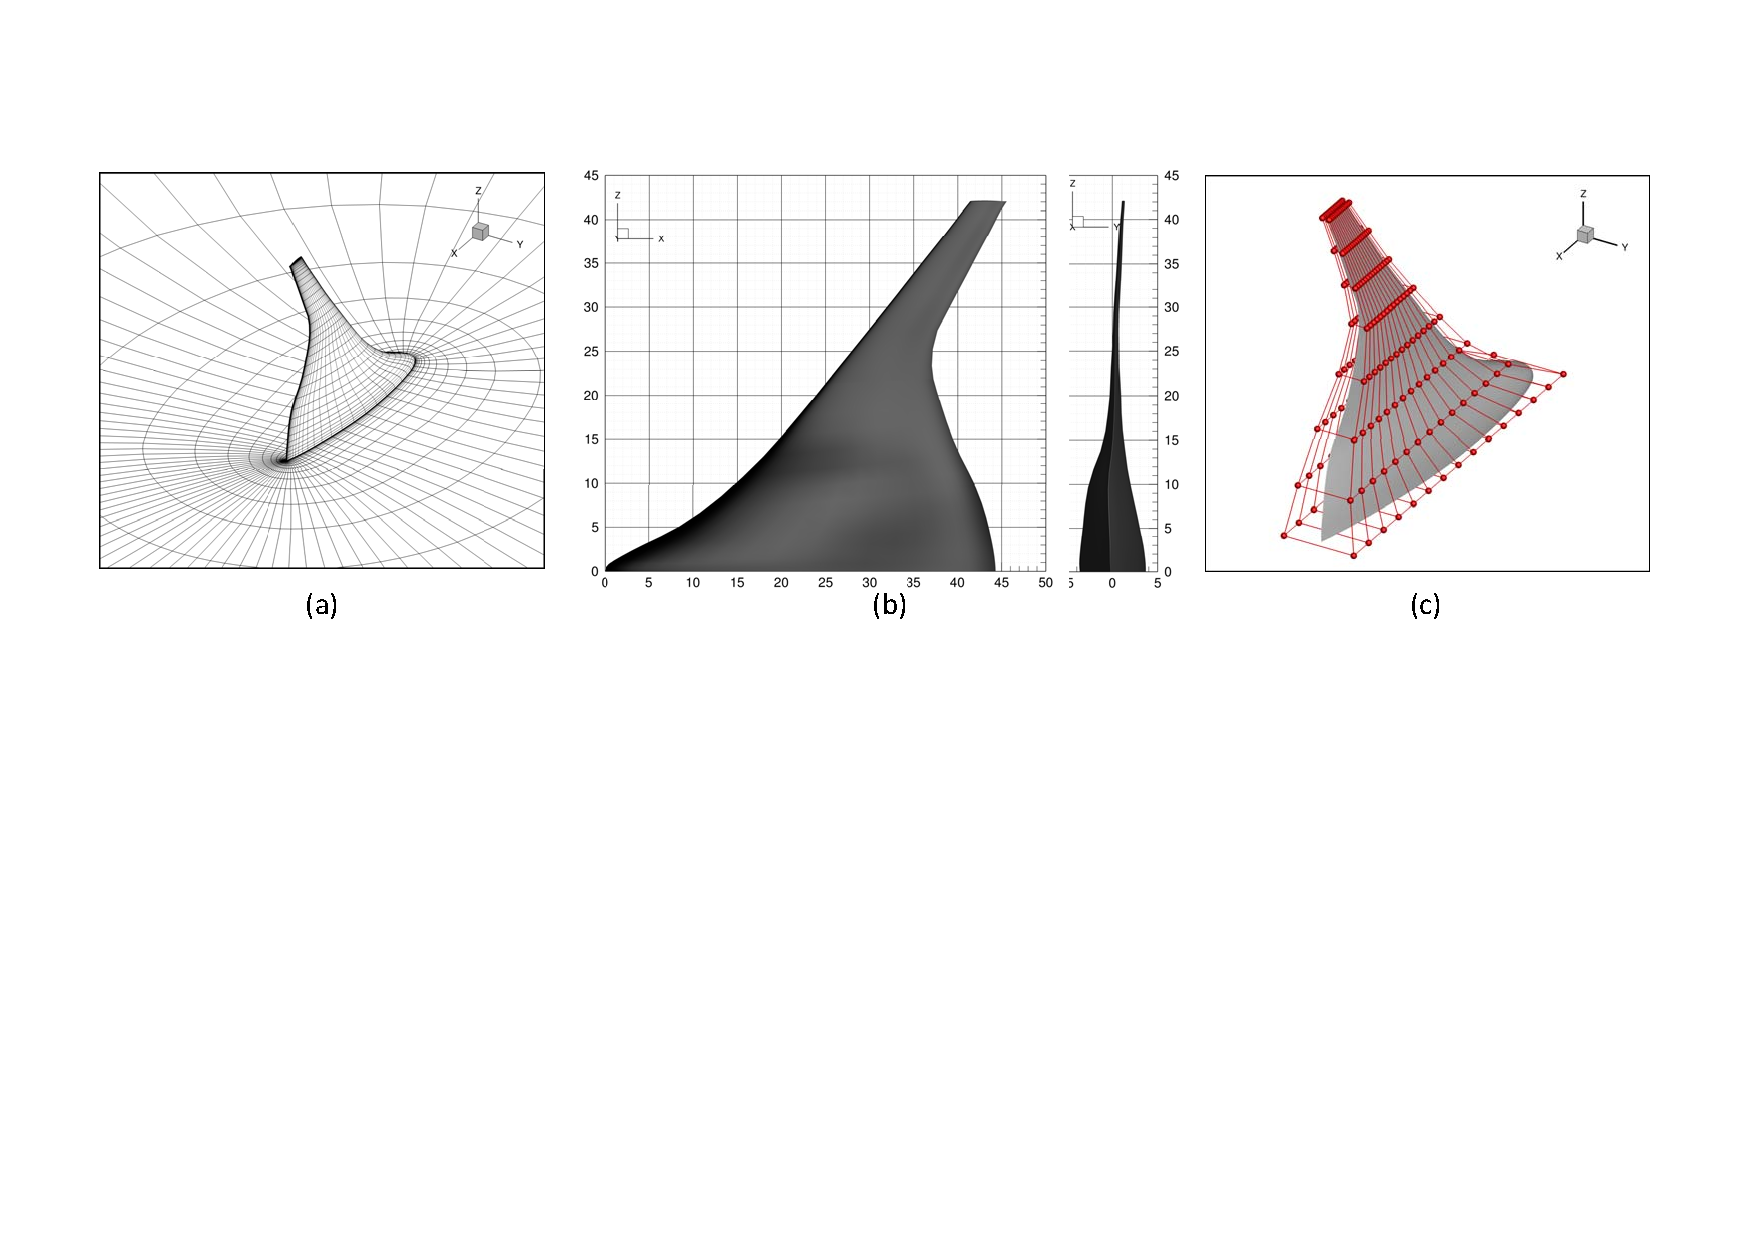
\includegraphics[width=1\linewidth]{chapter5/fig/bwb_template_mesh_initial_geometry.pdf}
    \end{center}
    \caption{
        \small Geometric setup for the BWB Case Study. (a) DeepGeo template mesh. (b) the initial BWB aircraft geometry and (c) the 240-point FFD setting.
    }
    \label{ch5:fig:cs3_template_mesh}
\end{figure}

\begin{figure}[htb]
    \begin{center}
        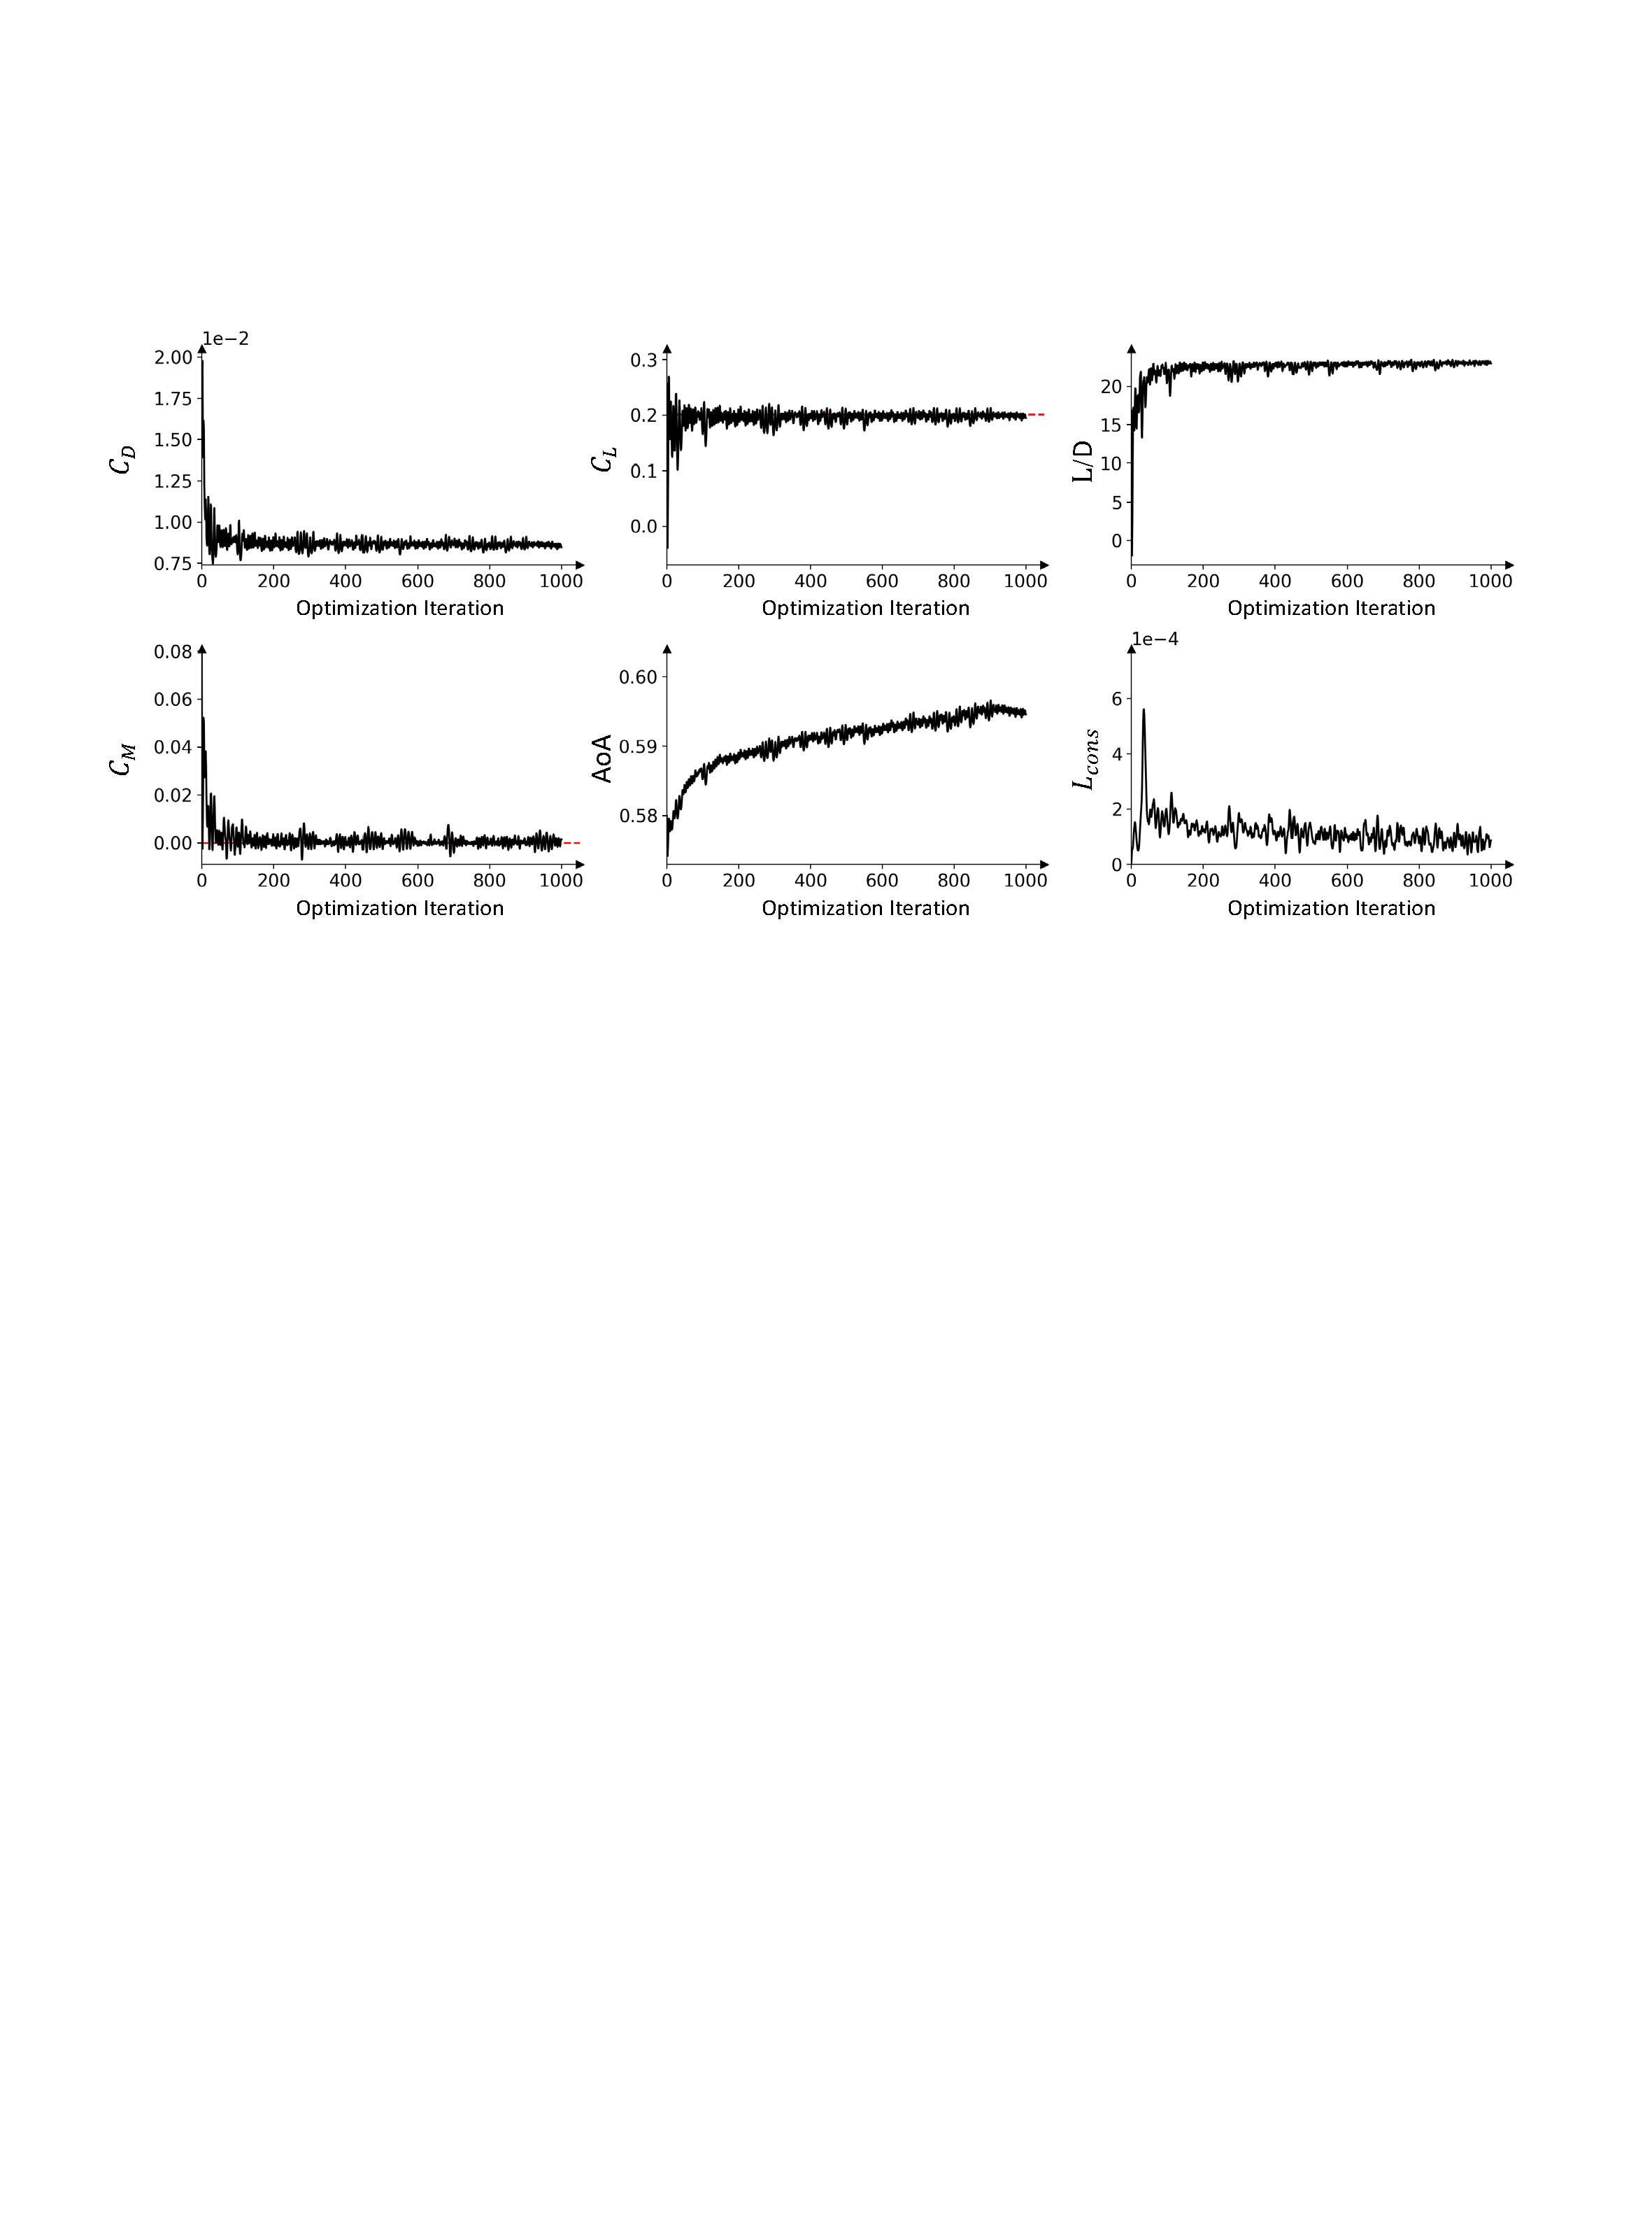
\includegraphics[width=1\linewidth]{chapter5/fig/bwb_L2_optim_history.pdf}
    \end{center}
    \vspace{-7mm}
    \caption{
        \small Evolution of important quantities during optimization for the BWB case. The dashed line in the $C_L$ and $C_M$ plots represent the optimization objectives.
    }
    \label{ch5:fig:cs3_history}
\end{figure}

\subsubsection{Configuring DeepGeo}

DeepGeo uses the L2 grid as template mesh. Similarly, DeepGeo parameterizes the BWB aircraft geometry through self-initialization, learning to generate all-zero deformation. 
Shape variations generated by DeepGeo are limited to the $z$ axis, in line with the allowed modifications specified by the optimization problem. This avoids the need for additional geometric constraints on the leading edge (LE) and trailing edge (TE).
The aerodynamic objective function $\cO_{CFD}$ and the volume constraint $\cL_{cons}$ from Eq.~\ref{ch5:eq:asoObj} are defined as
%
\begin{align}
 \cO_{CFD} &= \left| C_D \right| + \left| C_L-0.5 \right| + \left| C_M \right| \; , \\
 \cL_{cons} & = {\max \left(Vol(V^S)-{Vol}_\text{original}(S), 0\right)} ^2 \; .
\end{align}
%

\begin{figure}[!t]
    \begin{center}
        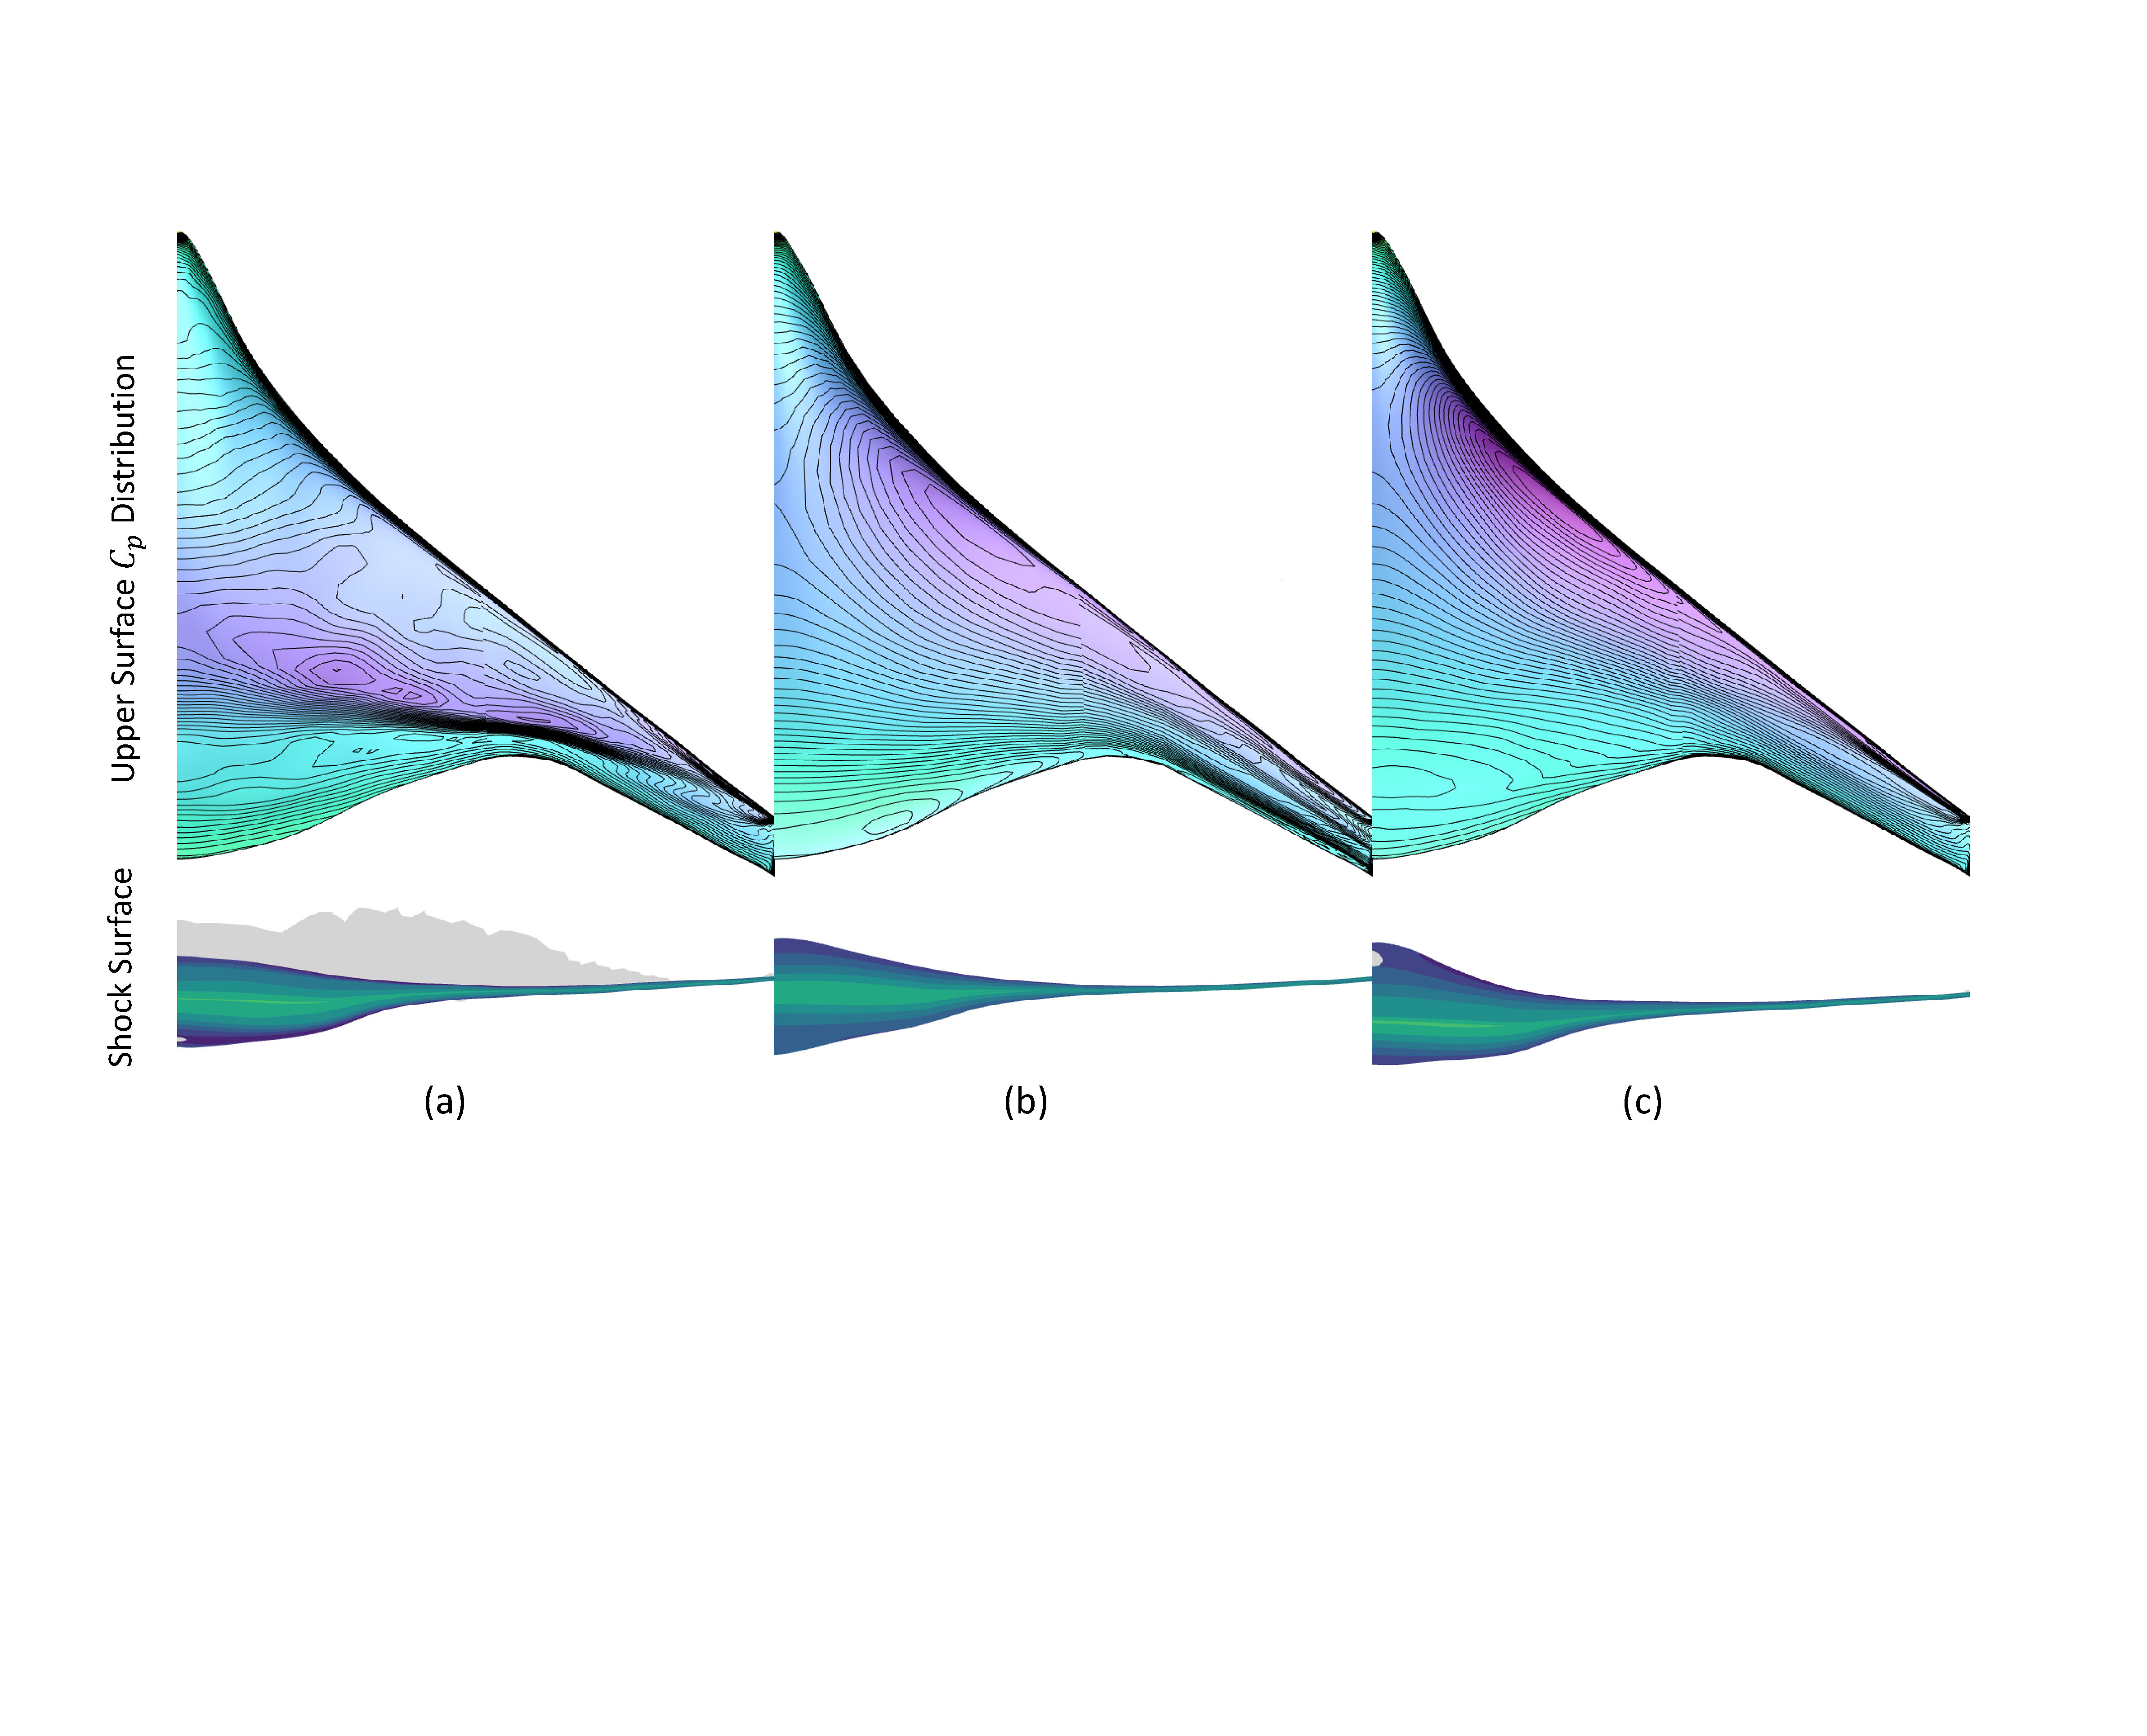
\includegraphics[width=1\linewidth]{chapter5/fig/bwb_optim_cp.pdf}
    \end{center}
    \caption{
        \small A comparison of Case Study III on the pressure coefficient distributions and shock shapes of (a) the initial CRM wing, (b) the wing optimized with 240-point FFD, and (c) the wing optimized with DeepGeo.
    }
    \label{ch5:fig:cs3_cp}
\end{figure}

\begin{figure}[!th]
    \vspace{2mm}
    \begin{center}
        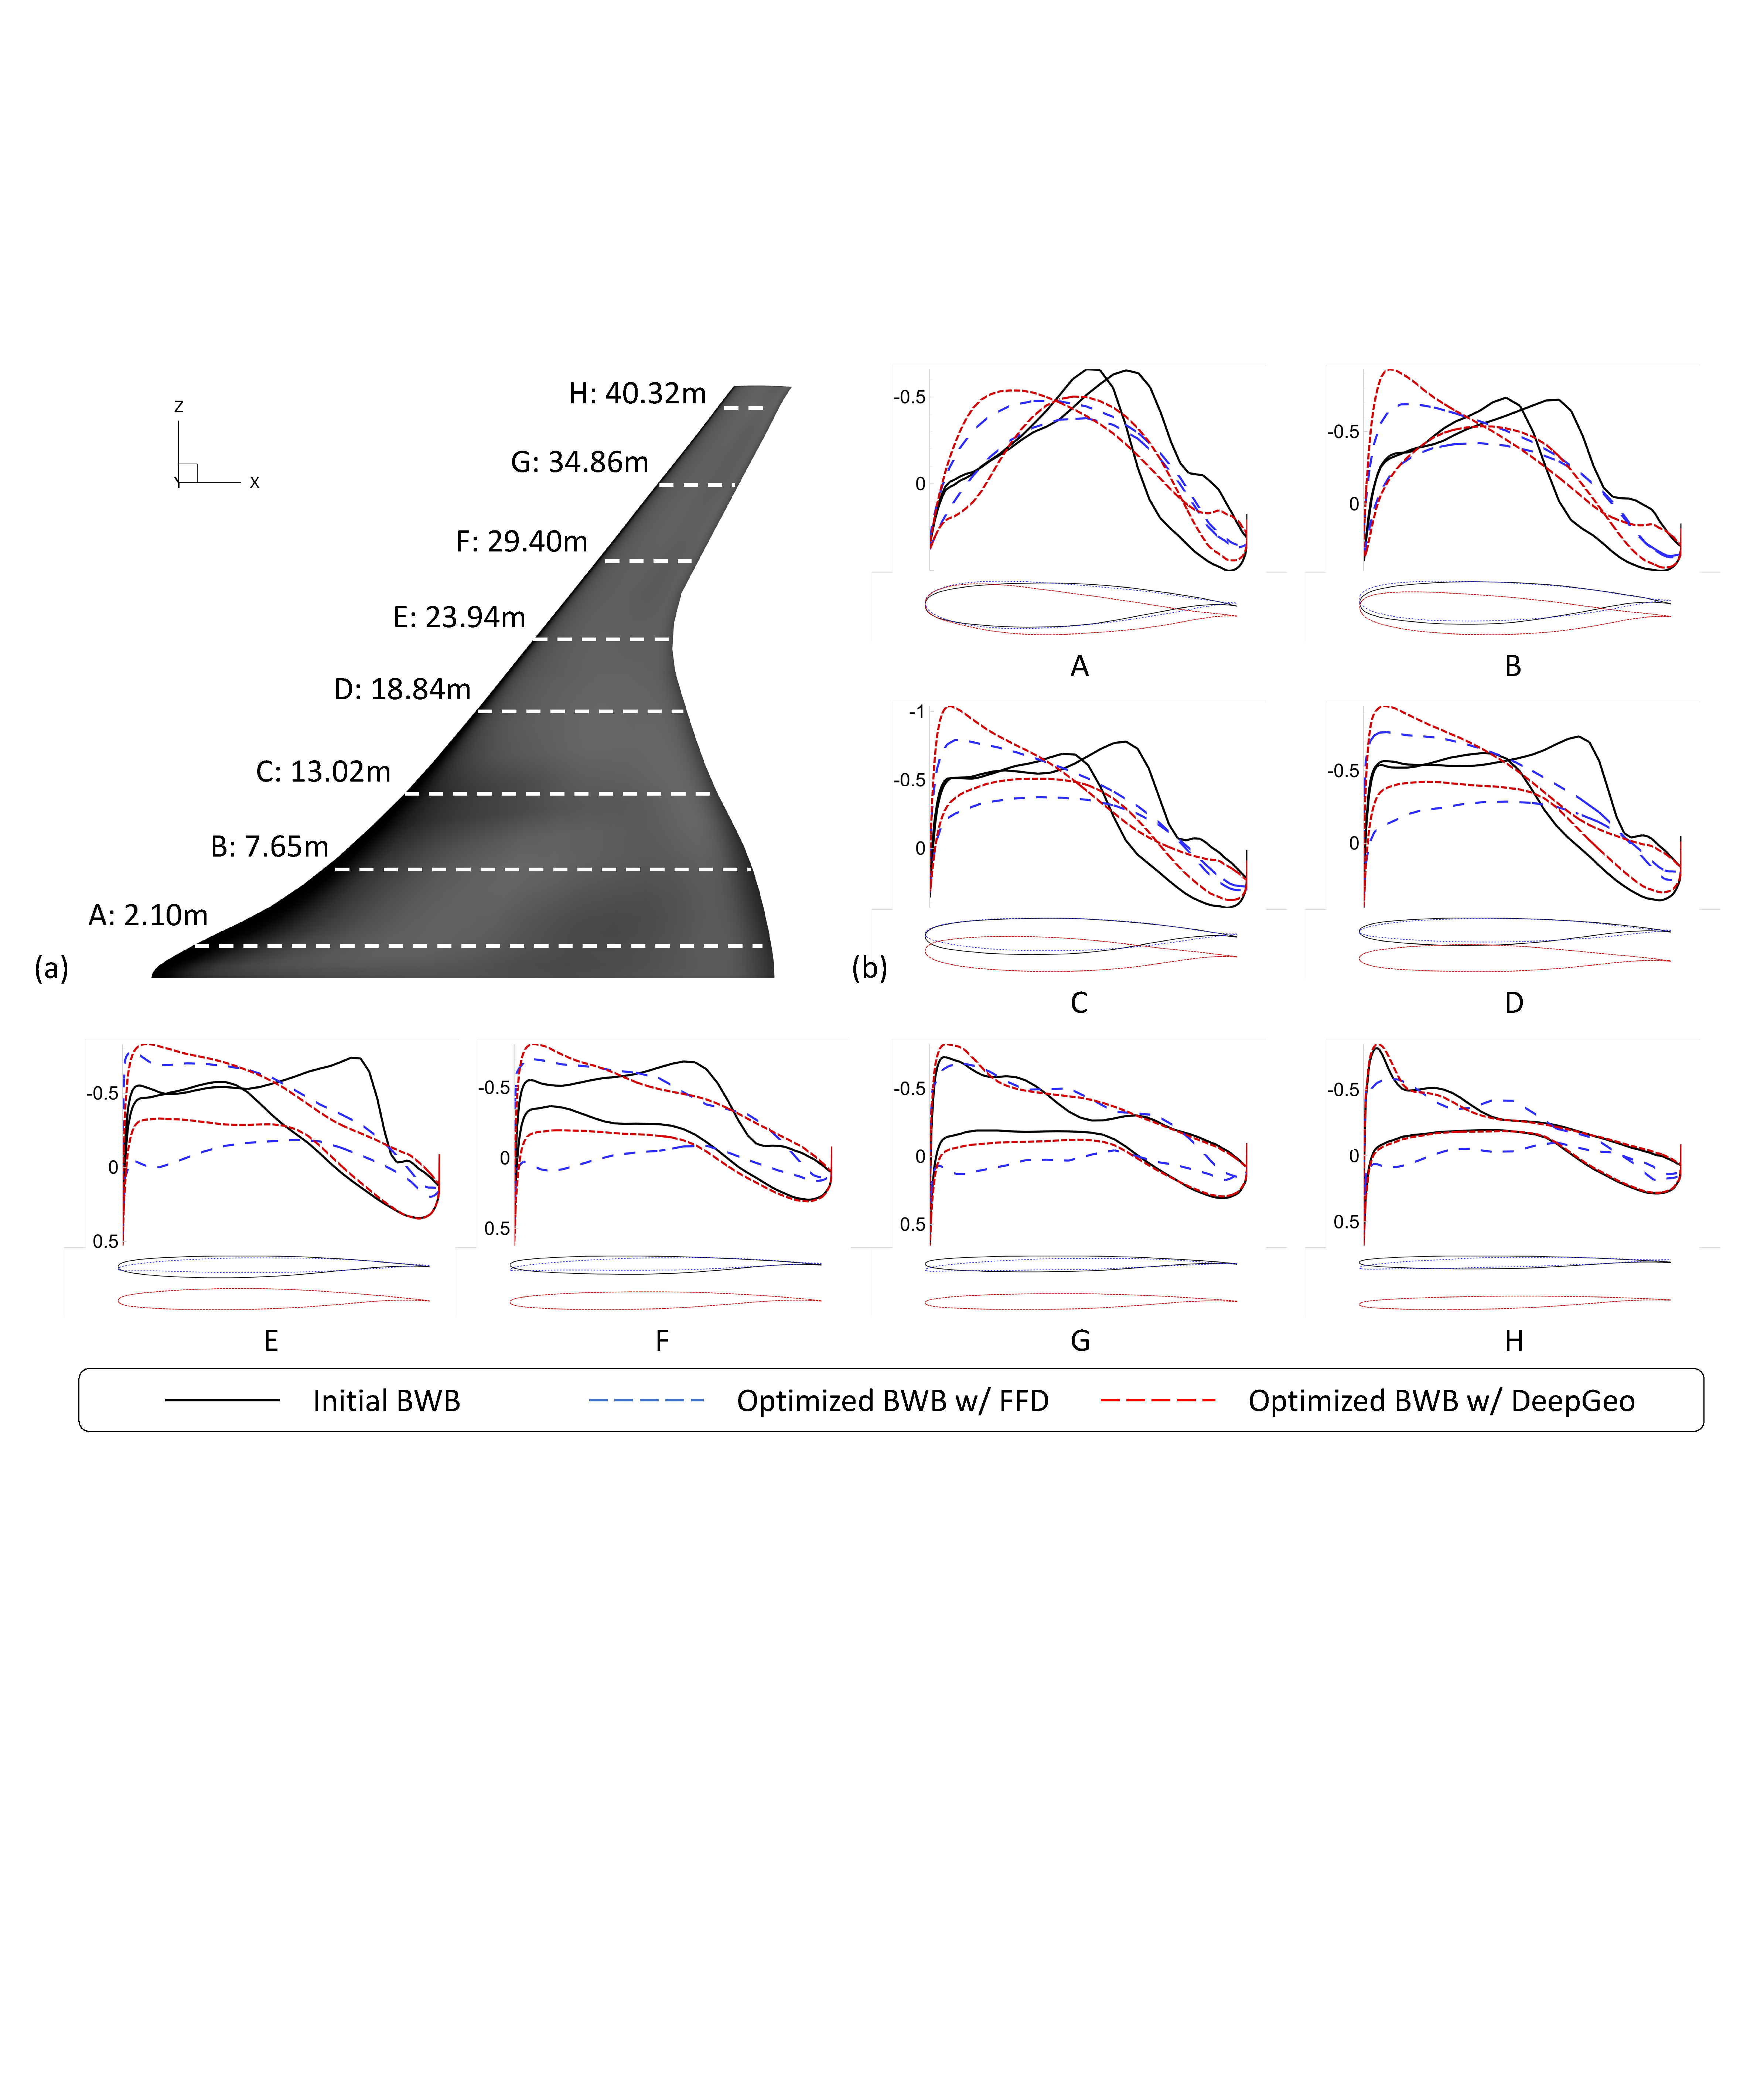
\includegraphics[width=1\linewidth]{chapter5/fig/bwb_optim_slice.pdf}
    \end{center}
    \caption{
        \small A comparison of Case Study III on sliced geometries, including (a) the positions of slices, and (b) the shape variation and pressure coefficient distribution of each slice.
    }
    \label{ch5:fig:cs3_slice}
\end{figure}

% \begin{table}[htbp]
%   \centering
%   \caption{BWB aircraft optimization results of the Case Study III.}
%     \begin{tabular}{l|ccccc}
%     \hline
%     \textbf{Parameterization} &  \multicolumn{1}{l}{\textbf{Final} $C_D$ {\footnotesize(counts)}} & \multicolumn{1}{l}{\textbf{Final} $C_L$} & \multicolumn{1}{l}{\textbf{Final} $C_M$} & \multicolumn{1}{l}{\textbf{Final} $\alpha$} & \multicolumn{1}{l}{\textbf{Final} {\footnotesize $Vol/Vol_\text{original}$}}\\
%     \hline
%     \multicolumn{6}{l}{\textbf{w/ L3 Grid}} \\
%     \hline
%     \textbf{DMM} & \num{104.14}  & \num{0.20055}  & \num{3.7524e-3}  & 0.60 & 99.1\%\\
%     \textbf{FFD} & \num{103.33}  & \num{0.20056}  & \num{-1.1998e-6} & 2.29 & \\
%     \hline
%     \multicolumn{6}{l}{\textbf{w/ L2 Grid}} \\
%     \hline
%     \textbf{DMM} & \num{86.42}  & \num{0.20072}  & \num{9.8807e-4} & 0.60 & 99.6\%\\
%     \textbf{FFD} &   &   &   &  & \\
%     \hline
%     \end{tabular}%
%   \label{tab:bwb_result}%
% \end{table}%

\begin{table}[!t]
  \centering
  \caption{\small BWB aircraft optimization results of the Case Study III.}
    \begin{tabular}{lcccc}
    \hline
    \textbf{Parameterization} &  \multicolumn{1}{l}{\textbf{Final} $C_D$ {\footnotesize(counts)}} & \multicolumn{1}{l}{\textbf{Final} $C_L$} & \multicolumn{1}{l}{\textbf{Final} $C_M$} & \multicolumn{1}{l}{\textbf{Final} $\alpha$}\\
    \hline
    \textbf{DeepGeo} & \num{86.42}  & \num{0.20072}  & \num{9.8807e-4} & 0.60 \\
    \textbf{FFD} & \num{87.05}  & \num{0.20056}  & \num{2.4675e-9}  & 2.47 \\
    \hline
    \end{tabular}%
  \label{ch5:tab:bwb_result}%
\end{table}%

\subsubsection{Configuring the Free-Form Deformation Baseline}

The FFD configuration follows the well-established settings proposed by~\citet{aa.Lyu2014}. This configuration uses 240 control points, as shown in Fig.~\ref{ch5:fig:cs3_template_mesh}(c). A minimal thickness constraint is added to prevent crashes caused by the negative volume error during optimization. The FFD baseline case uses IPOPT implemented in pyOptSparse~\cite{aa.Wu2020} for optimization.

\subsubsection{Results and Analysis}

Fig.~\ref{ch5:fig:cs3_history} shows the evolution of key aerodynamic quantities throughout the optimization process. The comparison with the FFD-based optimization history is provided in Appendix~\ref{ch5:sec:appendix_optim_history}. The optimization constraints on $C_L$ and $C_M$ are quickly fulfilled. The DeepGeo-based optimization achieves a shock-free design by the 149th iteration, and the number of total iterations remains within the same order of magnitude as the FFD-based optimization. Quantitative results comparing the automatic DeepGeo with the best manually configured FFD baseline are presented in Tab.~\ref{ch5:tab:bwb_result}. In terms of aerodynamic performance, DeepGeo achieves $47.8\%$ drag reduction in total and the drag performance is $0.63$ counts lower than FFD's result in $C_D$. Furthermore, as can be seen in Fig.~\ref{ch5:fig:cs3_cp}, the optimized FFD configuration exhibits a double shock near the wing tip, which is an undesirable feature in practical applications. In contrast, the DeepGeo-optimized design is shock-wave-free near the tip. 

Fig.~\ref{ch5:fig:cs3_slice}, provides a sectional analysis of geometry variations along the wingspan. The DeepGeo-optimized result shows more drastic changes in the spanwise bending and is less tilted upwards, while the shape variation on each slice is less significant. Similar to the results for the CRM wing, the FFD-optimized design has much sharper leading edges, which may negatively impact low-speed aerodynamic performance.

In summary, DeepGeo provides greater deformation freedom and, consequently, a broader design space for exploration when given less restrictive geometric constraints. In contrast, achieving similar flexibility with FFD requires users to manually implement various global design functions and introduce additional design variables, such as sweep, twist and dihedral functions, while carefully constraining each new design variable to avoid optimization failures. This approach requires significant additional engineering effort, making DeepGeo a more efficient and flexible alternative.